
%(BEGIN_QUESTION)
% Copyright 2009, Tony R. Kuphaldt, released under the Creative Commons Attribution License (v 1.0)
% This means you may do almost anything with this work of mine, so long as you give me proper credit

Read and outline the ``Cascade Control'' section of the ``Basic Process Control Strategies'' chapter in your {\it Lessons In Industrial Instrumentation} textbook.  Note the page numbers where important illustrations, photographs, equations, tables, and other relevant details are found.  Prepare to thoughtfully discuss with your instructor and classmates the concepts and examples explored in this reading.

\underbar{file i04336}
%(END_QUESTION)





%(BEGIN_ANSWER)


%(END_ANSWER)





%(BEGIN_NOTES)

Definition of cascade control: {\it when the output of one controller (primary, master) becomes the setpoint for another controller (secondary, slave)}.  An analogy for this is the delegation of work tasks from superior to subordinate.

\vskip 10pt

Control valve positioners are examples of cascade control: the positioner controls stem position according to the signal sent to it by the loop controller.  The loop controller is the master while the positioner is the slave.

\vskip 10pt

The slave loop in a cascade system must always be faster than the master loop, so that it will be able to follow orders from the master loop.  

\vskip 10pt

The example air dryer cascade system quickly compensates for loads by slave loop controlling inlet air temp.  If load changes, this inlet air temp will be corrected by the slave controller before any effect ever reaches the master controller's transmitter.  The slave controller thus ``shields'' the master controller from having to deal with loads.

The example boiler feedwater cascade system compensates for loads by a slave loop controlling feedwater flow into the drum.  If a load on the feedwater system changes, this inlet feed flow will be corrected by the slave controller before any effect is seen in drum level.  Once again, the slave controller ``shields'' the master controller from having to deal with loads.  Any problems with valve characterization become the flow controller's problem, not the level controller's problem.

The example servo motor system is a triple-cascade loop: position to velocity to acceleration.  Without cascading, a single PID controller would see the platform position as a runaway process.  With cascade control, the characteristic becomes integrating instead, which is easier to control.

\vskip 10pt

Slave loop must be tuned before the master loop is tuned, due to the dependence of the master controller on the slave controller's robust behavior.







\vskip 20pt \vbox{\hrule \hbox{\strut \vrule{} {\bf Suggestions for Socratic discussion} \vrule} \hrule}

\begin{itemize}
\item{} Explain why cascade control strategies are employed in some processes.
\item{} Explain how a valve positioner is an example of a cascade control loop.
\item{} Explain how cascade control ``shields'' one of the controllers from certain loads.  Which controller (master or slave) is being shielded by the other?  Illustrate this concept by applying it to an example control system, such as one of those highlighted in the book.
\item{} Choose any one of the cascade control examples shown in the textbook and identify some process loads that are {\it not} compensated for by the slave loop.
\item{} Identify how the control loop you built in your lab project might possibly benefit from cascasde control.
\item{} For those who have studied control valves, explain how a cascaded flow control (slave) loop helps to overcome poor valve sizing and/or characteristic problems that would otherwise plague the stability of the master loop.
\item{} For those who have studied process characteristics, explain how a slave loop may favorably alter the characteristics of the process as seen by the master controller.
\item{} Explain in your own words exactly why the slave loop must be tuned first in a cascade control system.
\item{} Perform fault analysis on any of the cascade control loops shown in the chapter: propose a fault, and have students predict the effects.  Examples include:
\begin{itemize}

\item{} Heat exchanger in dryer system becomes fouled with dust
\item{} Feedwater pump speeds up in boiler system
\item{} Air signal tube between LIC and FIC in boiler system breaks open
\item{} Hall effect sensor in motion control system fails with zero signal
\item{} Tachogenerator in motion control system fails with zero signal
\item{} Position sensor in motion control system fails with high signal
\end{itemize}
\end{itemize}







\vfil \eject

\noindent
{\bf Prep Quiz:}

{\it Cascade} control loops typically have:

\begin{itemize}
\item{} Multiple transmitters, one controller, and one final control element
\vskip 5pt 
\item{} One transmitter, one controller, and one final control element
\vskip 5pt 
\item{} Multiple transmitters, multiple controllers, and multiple final control elements
\vskip 5pt 
\item{} One transmitter, one controller, and multiple final control elements
\vskip 5pt 
\item{} One transmitter, multiple controllers, and multiple final control elements
\vskip 5pt 
\item{} Multiple transmitters, multiple controllers, and one final control element
\end{itemize}



\vfil \eject

\noindent
{\bf Prep Quiz:}

In a {\it cascade} control loop, you typically need to tune:

\begin{itemize}
\item{} Nothing at all, because cascade loops are inherently self-tuning
\vskip 5pt 
\item{} The slave controller first, because the master controller depends on it to control well
\vskip 5pt 
\item{} The transmitter first, because its PID parameters must be proper for anything to work
\vskip 5pt 
\item{} The slave controller first, because it is generally simpler to tune than the master
\vskip 5pt 
\item{} The master controller first, because the slave controller depends on it to control well
\vskip 5pt 
\item{} The master controller first, because it is generally simpler to tune than the slave
\end{itemize}


\vfil \eject

\noindent
{\bf Summary Quiz:}

Identify the proper actions for each of the controllers in this cascade system, assuming direct-acting transmitters and an air-to-open control valve:

$$\includegraphics[width=15.5cm]{i04336x01.eps}$$

Master (TC-1a) = {\it direct} or {\it reverse}?

\vskip 10pt

Slave (TC-1b) = {\it direct} or {\it reverse}?

%INDEX% Reading assignment: Lessons In Industrial Instrumentation, basic control strategies (cascade)

%(END_NOTES)


